\documentclass[../document]{subfiles}

\begin{document}
\subsection{Requirements Cast 2}
\subsubsection{Introduction}
We are using the goal driven requirement development method to gather our requirements. The first part of this document will be a top down goal level view, with a main goal and sub goals. The second part gives a more detailed textual description for some of the important requirements, followed by a table with a short description for each functional requirement. Eventually part three presents pictures and textual descriptions showing each of the three different views that we will implement.

\subsubsection{Top goal of the system}
\begin{itemize}
	\item
	Gather data and present the data visually
	\begin{itemize}
		\item
		Data storage requirement
		\begin{itemize}
			\item
			Storing data
			\item
			Pull data
		\end{itemize}
		\item
		Central hub requirement
		\begin{itemize}
			\item
			Gather data from sensor
			\item
			Send data upon request
		\end{itemize}
		\item
		Client requirement
		\begin{itemize}
			\item
			Pull data from central hub
			\item
			Process data
			\item
			Store processed data in the database
		\end{itemize}
		\item
		Visualizer requirement
		\begin{itemize}
			\item
			Pull data from the database
			\item
			Show the data on the GUI
			\begin{itemize}
				\item
				Show a table containing sensors and their data values
				\item
				Show a map with sensors and their position if possible
				\item
				Map will showcase the temperature, humidity, pressure, sound and lighting near the sensor
			\end{itemize}
			\item
			Allow user to manipulate historical data
			\begin{itemize}
				\item
				A button will lead to a pop out window containing historical data (in other words data averaged out over one day) in a list.
			\end{itemize}
			\item
			Allow the user to switch to different data types
		\end{itemize}
	\end{itemize}
\end{itemize}

\subsubsection{Database interaction requirement}
There will be a database where the data collected from the sensors is stored. The data will include time of recording, sensor identification, location if applicable, and measured values such as temperature and lighting. The data can be pulled out later by other modules to be used. 

\begin{table}[H]
\caption{Database interaction requirement}
\centering
\begin{tabularx}{\textwidth}{|l|X|X|l|X|}
\hline
\\ \hline Req.nr
&Name
&Description
\\ \hline 1.1
&Storing data
&The client can push data into the database
\\ \hline 1.2
&Pull data
&The visualizer can pull data out of the database
\\ \hline 
\end{tabularx}
\end{table}

\subsubsection{Central hub requirement}
The main task of the central hub is to gather the information and send it to the client when requested. The central hub consist of hardware and software. The hardware part is the sensor itself. Because this is provided by the customer, the requirement part is not necessary. The software server will function as a gather and send unit, which gathers data from the sensors and forwards the data if requested.

\begin{table}[H]
\caption{Central hub requirement}
\centering
\begin{tabularx}{\textwidth}{|l|X|X|l|X|}
\hline
\\ \hline Req.nr
&Name
&Description
\\ \hline 2.1
&Gather data from sensor
&The sensor data will be collected by the server.
\\ \hline 2.2
&Send data upon request
&If the central hub gets a request to send data from the client, it will send the data.
\\ \hline 2.3
&Support hotjoin
&Sensors should be able to disconnect and connect to the central hub at will.
\\ \hline 
\end{tabularx}
\end{table}

\subsubsection{Client requirement}
The main task of the client is to take the data from the central hub and store it into the database. The client will send requests to the central hub and get sensor data in that way. The client can process data into strings for storage that the client will store in the database.

\begin{table}[H]
\caption{Client requirement}
\centering
\begin{tabularx}{\textwidth}{|l|X|X|l|X|}
\hline
\\ \hline Req.nr
&Name
&Description
\\ \hline3.1
&Pull data from central hub
&The client will send a pull data request to the central hub which will result in the central hub sending back gathered sensor data.
\\ \hline3.2
&Process data into strings
&The data will be processed into strings.
\\ \hline3.3
&Store data in the database
&After processing the data, the client will store it into the database.
\\ \hline 
\end{tabularx}
\end{table}

\subsubsection{Visualizer requirement}
The visualizer is the main focus of the project. As a result of that this is also the part with most requirements. The visualizer will first gather the data it needs from the database, then present it on a map featuring the position to each sensor. The map will also show the temperature, humidity, pressure, sound and lighting near the sensor. We will also create multiple types of views.

\begin{table}[H]
\caption{Central hub requirement}
\centering
\begin{tabularx}{\textwidth}{|l|X|X|l|X|}
\hline
\\ \hline Req.nr
&Name
&Description
\\ \hline 4.1
&Pull data from the database
&The visualizer will be able to pull whatever data it desires.
\\ \hline 4.2
&Show the data on the GUI
&The data will be displayed in a window.
\\ \hline 4.2.1
&Present data in a table
&The data collected will be placed in a table with each data type having its own column.
\\ \hline 4.2.2
&Present data in a map with sensors
&We will construct a map containing sensors and possibly their position. The data, such as temperature, will be displayed near each sensor.
\\ \hline 4.3
&View historical data
&The user should be able to view historical data.
\\ \hline 4.3.1
&Allow the user to see views with historical data
&The user will be able to click on a button to see data recorded earlier.
\\ \hline 4.3.2
&Graph view
&The user should be able to view a graph of the data over time.
\\ \hline 4.4
&Allow the user to switch between different data type
&The user should be able to select what kind of data type they want to see in order to not clutter the screen with data the user is not interested in.
\\ \hline 
\end{tabularx}
\end{table}

\subsubsection{Table view}
This is the view where all sensors and the data is showcased in a table. The sensor number can be seen on the left and what data they are gathering. If the user prefers less information, the checkboxes can be check or unchecked to show or hide the data.

\begin{figure}[H]
	\centering
	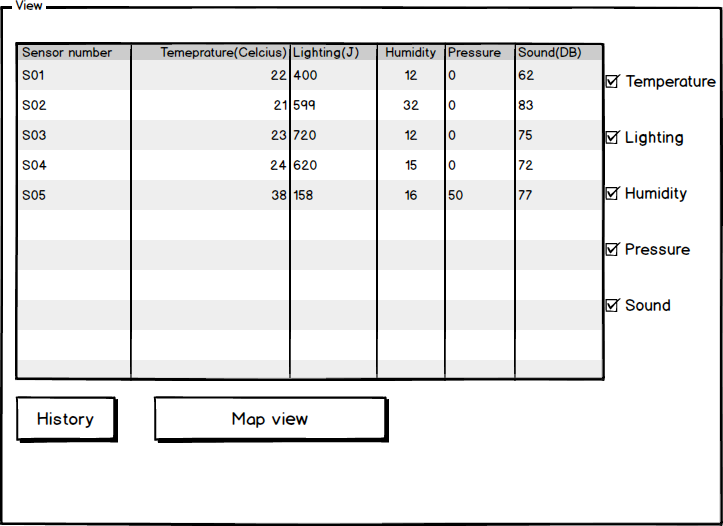
\includegraphics[width=\textwidth]{retierd_requirements/Table_view.png}
	\caption{Table view}
\end{figure}

\subsubsection{Map view}
The map view will make an illustration of the room. In the real model the data will be shown in the form of image manipulation, not a function in the mockup program. We will track the position of the sensors and show the data in a 2D map.

\begin{figure}[H]
	\centering
	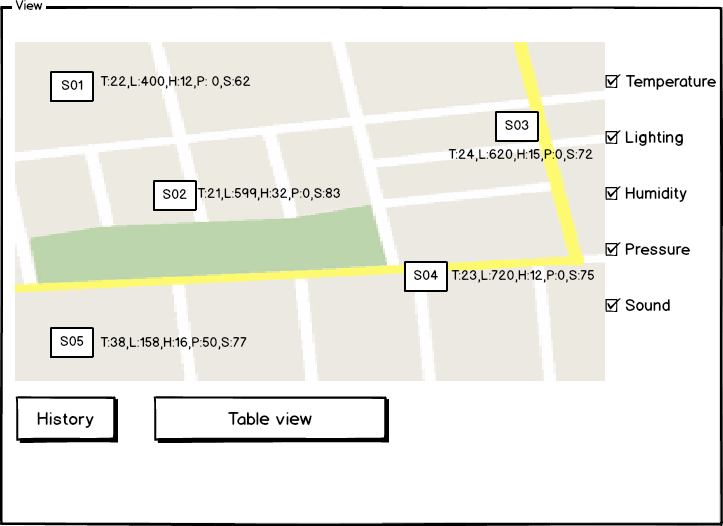
\includegraphics[width=\textwidth]{retierd_requirements/Map_view.png}
	\caption{Map view}
\end{figure}

\subsubsection{History view}
The user can also access the historical data that is saved in the database by clicking on the history button. A list of data that is recorded will then pop up and by selecting one of them, you get to see the data of that specific time. You can close this mode if you click on the current button or close the history data window.

\begin{figure}[H]
	\centering
	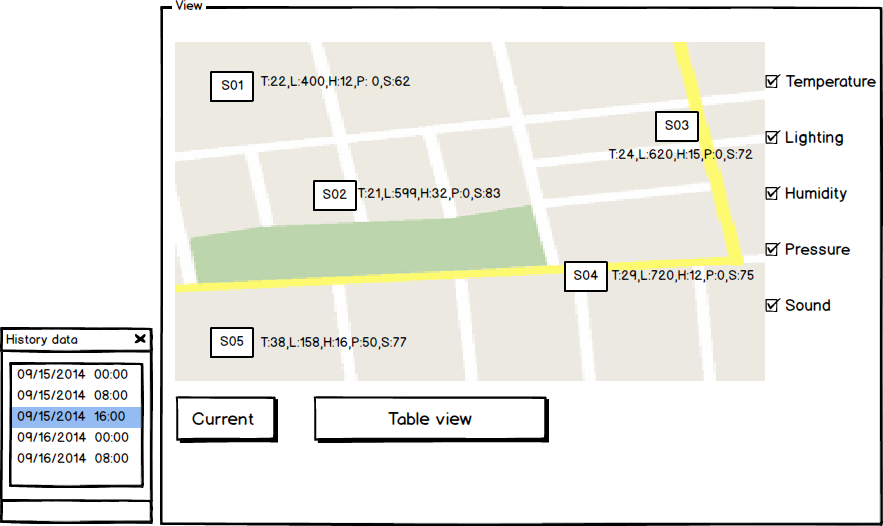
\includegraphics[width=\textwidth]{retierd_requirements/History_view.png}
	\caption{History view}
\end{figure}

\end{document}